\chapter{Metodologia}
\label{chap:metodologia}

Abans de començar a escriure cap línia de codi cal determinar quina és la metodologia que s'utilitzarà durant el projecte. 

Així en aquest s'ha utilitzat el model incremental o iteratiu. A més a més s'ha complementat amb la utilització de Test Driven Development i el Behaviour Driven Development per poder controlar de forma automatitzada el correcte funcionament de l'aplicació i que aquesta es comporta de tal i com s'sesperació.

En els següents apartats es descriu amb més detalles les característiques d'aquestes metodologies.  

\section{Model Incremental o Iteratiu}

Per a la realització de tot el software relacionat amb el projecte s’ha utilitzat un model de procés del software incremental. Aquest model aplica seqüències lineals de forma esglaonada a mesura que avança el temps. Per tal d'aconseguir això es divideix el projecte en diferents funcionalitats, que s'implementen una radere de l'altra formant iteracions. Cada vegada que es finalitza una iteració es produeix un \emph{increment} en el software. Cada increment o iteració és compon de les següent fases: anàl·lisis, disseny, codificació i proves. A la figura \ref{fig:mii} es pot veure un diagrama del cicle de desenvolupament del model incremental.

\begin{figure}[htbp]
\centering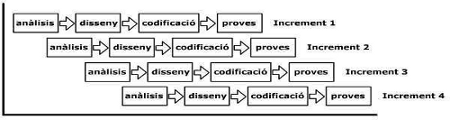
\includegraphics[width=12cm]{img/model-incremental.png}
\caption{Cicle de desenvolupament del model incremental.}
\label{fig:mii}
\end{figure} 

Quan es finalitza un increment el software es mostra al usuari amb l'objectiu de validar que cumpleix amb les espectatives desitjades. A més a més, el software ha de ser verificat i testat en cada increment. Això ens permet evitar l'acumulació d'errors en els pròxims increments. És un model molt útil quan volem anar entregant fases incompletes del sistema per tal que els usuaris les puguin anar provant, i així, inclús podem afinar més en l’anàlisi dels requiriments de les pròximes iteracions.

Els avantatges d’utilitzar aquest model són:

\begin{itemize}
\item{Té en compte l’evolució del software.}
\item{Els primers increments permeten descobrir nous requeriments per a pròxims increments.}
\item{El client aviat rep versions operatives (encara que incompletes) del producte, i en conseqüència s’involucra més en el procés.}
\item{Funciona bé quan l’equip de programadors es reduït.}
\end{itemize}

Els inconvenients d’utilitzar aquest model són:

\begin{itemize}
\item{Problemes per determinar les funcionalitats a desenvolupar a cada increment.}
\end{itemize}


\section{Test Driven Development}
\label{sec:tdd}

Test Driven Development o desenvolupament de software bastat en Testos és una metodologia de desenvolupament de software centrada en els jocs de proves. Un joc de prova és un executable que s'utilitza per comprovar de forma automàtica que el que es vol implementar compleix amb les funcionalitats i els requeriments disenyades en la fas d'anal·lisi. Per tal d'aconseguir-ho cada un dels jocs de proves s'associa amb les especificacions del que es vol contruir. Això ens permet validar de forma automàtica que el que s'ha contruït compleix amb les especificacions o requeriments desitjade. A la figura \ref{fig:tdd} es pot veure un diagrama del cicle de desenvolupament basat en Test Driven Development.

\begin{figure}[htbp]
%\centering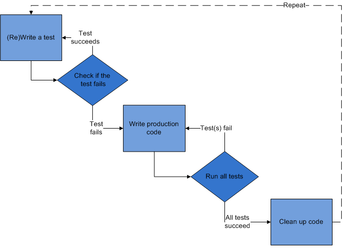
\includegraphics{img/test-driven-development.png}
\centering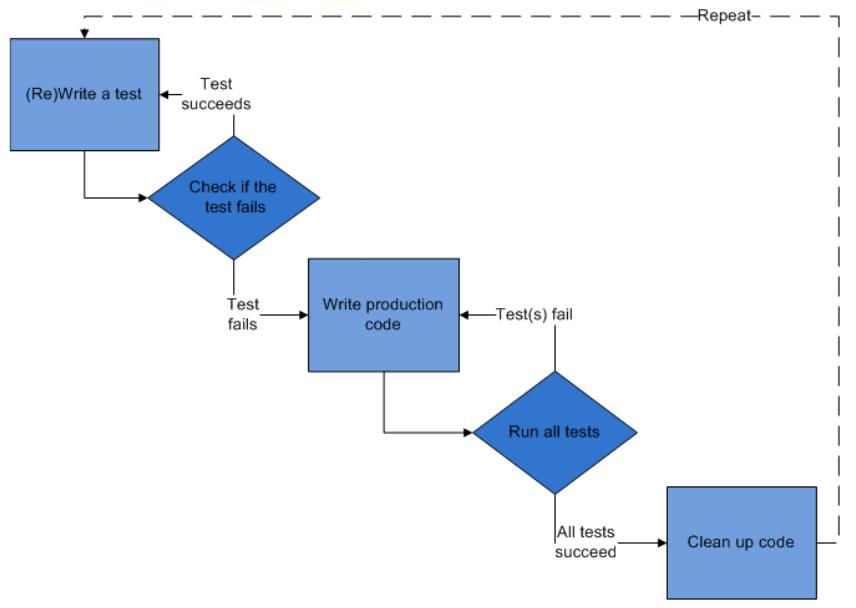
\includegraphics[width=12cm]{img/ttd1.jpg}
\caption{Representació del cicle de desenvolupament basat amb TDD}
\label{fig:tdd}
\end{figure} 

\newpage

Aquesta metodologia utilitza el següent cicle de desenvolupament: 

\begin{enumerate}
    \item{Escriure un joc de prova.}
    \item{Executar tots els jocs de prova per comprovar que el nou test falla.}
    \item{Escriure el codi necessari per a que el joc de prova sigui favorable.}
    \item{Executar tots els jocs de provar per comprovar que tots els test són satisfactoris.}
    \item{Reestructurar el codi}
\end{enumerate}

Aquesta metodologia té l'objectiu d'implementar petites funcionalitats que puguin ser provades de forma independent per un joc de prova, per tal de desprès ajuntar-les amb el conjunt de l'aplicació. Gràcies a això s'aconsegueix millorar l'àmbit de proves de l'aplicació, ja que cada funcionalitat es prova dos vegades: una per separat i una altra amb el conjunt de tota l'aplicació.  

El Test Driven Development té les següents ventatges: 

\begin{enumerate}
    \item{Major flexiblitat del codi, ja que per poder ser testejat aquest ha de funcionar de forma independent i en el conjunt de tot l'aplicació.}
    \item{Claredat dels requisits a implementar.}
    \item{Millora de la productivitat, ja que es garanteix que el codi que s'ha escrit funciona.}
    \item{Major seguretat en vers a l'evol·lució, ja que al testejar el codi s'obté més confiança a l'hora de canviar-lo.}
\end{enumerate}

i els següents inconvenients: 

\begin{enumerate}
    \item{Difícil d'implementar en alguns casos: Interfícies de client,bases de dades, programes dependents de la xarxa.}
    \item{Dependència de que els testos estiguin ben escrits. }
\end{enumerate}

\section{Behavoir Driven Development}
\label{sec:bdd}

El Behavoir Driven Development és una extensió del Test Driven Development en la qual s'utilitzen els jocs de proves per 
especificar el comportament que ha de tenir el sistema en determinades ocasions. Això permet que els desenvolupadors es concentrin en perquè el codi ha d'estar creat i no tan en els detalls tècnis. També permet minimitzar les diferències entre el llenguatge en que està escrit el codi i el llenguatge utiltizat pels usuaris del sistema. 

